\section{Isomorphism}


\subsection{Problem definition}
In the isomorphism problem we have to determine for two given graphs $G$ and $H$ if there exists a bijection $\phi$ from $V(G)$ to $V(H)$ such that $\forall u, v \in V(G), \ \{u, v\} \in E(G) \iff \{\phi(u), \phi(v)\} \in E(H)$.

\subsection{Parameterized complexity}
In classical complexity we only take into account the length of the input to study the complexity of a problem. Unfortunately, many problems become intractable under this measure with the best algorithms we know. This is the case of both the famous NP-complete problems and the graph isomorphism problem. The fastest know exact algorithms for these run in exponential and sub-exponential time respectively. 

In parameterized complexity on the other hand, we don't only take into account the size of the input, but also a parameter about the input, e.g the tree depth of the input graph in the isomorphism problem. An interesting complexity class is the Fixed Parameter Tractable. We consider a problem to be in this class, if we can find a solution in time @@TODO O($f(d) * n$), where $n$ is the size of the input, $d$ is the parameter and @@TODO $f: N -> N$. Beware, that such a function can be exponential or even worse.

In this chapter we will show that such an algorithm exists for the isomorphism problem parameterized by the tree depth of the graphs. This means that we can solve the problem for any class of graphs with a bounded tree depth in polynomial time with respect to their size.

\subsection{Bounded roots}

\begin{definition}
Let G be a connected graph with tree depth $d$. Then, root($G$) = $\{ v \in G$ : $td(G - v) = d - 1\}$ is the set of roots of $G$.
\end{definition}

For the algorithm we will need to proof that $|root(G)|$ is bounded by a function of the tree depth of $G$. Still, this is not a simple proof and we will need to introduce new concepts and lemmas.

\begin{definition}
Let $G$ be a connected graph and $B$ a subset of the nodes of $G$. For two connected components of $G \setminus B$, $C_1$ and $C_2$, we will say $C_1$ and $C_2$ are equivalent in $G$ with respect to $B$ if and only if the following holds: \\
There exists a bijection $\Phi : C_1 \cup B \longrightarrow C_2 \cup B$ such that $\forall b \in B$, $\Phi (b) = b$ and $\forall u, v \in V(C_1) \cup V(B)$, $\{u, v\} \in E(G) \iff \{\Phi (u), \Phi (v) \} \in E(G)$.
\end{definition}

We can visualize this equivalence relation as two components being isomorphic and connected in the same way to the set $B$.

\begin{example}
Let the graph in the image be $G$ and $B = \{\alpha, \beta \}$. The component of the node $\delta$ in $G \setminus B$ and the one of node $\epsilon$ are equivalent with respect to $B$, but they are not equivalent to the one consisting of $\gamma$.
\begin{figure}[!h]
\centering
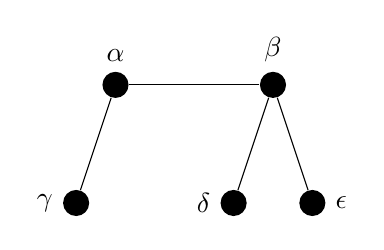
\begin{tikzpicture}
\node [label=above:{$\beta$}, fill=black, circle] (v2) at (-2,1) {};
\node [label=above:{$\alpha$},fill=black, circle] (v1) at (-4,1) {};
\node [label=left:{$\gamma$},fill=black, circle] (v3) at (-4.5,-0.5) {};
\node [label=left:{$\delta$}, fill=black, circle] (v4) at (-2.5,-0.5) {};
\node [label=right:{$\epsilon$}, fill=black, circle] (v5) at (-1.5,-0.5) {};
\draw  (v1) edge (v2);
\draw  (v1) edge (v3);
\draw  (v2) edge (v4);
\draw  (v2) edge (v5);
\end{tikzpicture}
\end{figure}
\end{example}

\begin{lemma}
Let $G$ be a connected graph with td($G$) = $d$ and $B$ a subset of the nodes of $G$. Let $C_1$, $C_2$, $\dots$, $C_k$ be equivalent components in $G$ with respect to $B$. Let $G'$ be the graph left after we remove all the $C_i$ with $i > d + 1$. Then, td($G$) = td($G'$) and root($G$) = root($G'$).
\label{lemma:equiv-comps}
\end{lemma}
\begin{proof}
@@TODO
\end{proof}

\subsection{Bounded roots in minimal graphs}
\begin{definition}
We will say a graph $G$ with td($G$) = $d$ is a minimal graph if for any subset of its nodes $B$, it has at most $d + 1$ equivalent components in $G$ with respect to $B$. 
\end{definition}

We are interested in minimal trees because of the following lemma.

\begin{lemma}
For any graph $G$, there exists a graph $G'$ such that root($G$) = root($G'$), td($G$) = td($G'$) and $G'$ is minimal.
\end{lemma}
\begin{proof}
@@TODO
\end{proof}

By using this lemma, we only have to proof that the number of nodes is bounded  by the tree-depth in minimal graphs. This is easy to see, because for any graph, there exists a minimal graph with the same roots and tree-depth. As the roots are a subset of the nodes, proving that the set of nodes is bounded is sufficient.

\begin{lemma}
Let $G$ be a minimal graph with td($G$) = $d$. Then, there exists $f(d, i)$ such that it returns the maximum possible size of the graph left after $i$ rounds of the $d$-selection-deletion game.
\end{lemma}
\begin{proof}
We will proof this by reverse induction on $i$.
\begin{itemize}
%@@TODO: check alice
  \item \textbf{Base case}: If $i = d$, then clearly $f$ exists. $f(d, i)$ = 0, because otherwise Alice would have winning strategy in the $d+1$-selection-deletion game and td($G$) would be higher than $d$, a contradiction.
  \item \textbf{Induction}: If $i < d$, we can assume $f(d, k)$ exists for all $k > i$. Let $B$ be the set of nodes that Bob has removed in the first $i$ rounds of the game. We know that the size of each component of $G \setminus B$ is at most $s = f(d, i+1)$, because Alice will pick a component of $G \setminus B$ for the round $i+1$ and Bob can only remove a node. There are less than $2^{s^2}$ isomorphic graphs of size $s$. Each of this graphs can be connected to $B$ in $2^{i \cdot s}$  different ways, because each node in the component can have an edge to each node in $B$. With all this we can calculate the total number of equivalent components with respect to $B$, $s' = 2^{s^2} \cdot 2^{i \cdot s} = 2^{s^2 + i \cdot s}$. Because $G$ is minimal, we know that each equivalent component will appear at most $d + 1$ times. Thus, $f(d, i) = 1 + (d+1) \cdot s'$.
\end{itemize}
\end{proof}

With this last lemma, we know that any minimal graph $G$ with td($G$) = $d$ will have at most $f(d, 0)$ nodes. As we showed earlier this result also generalizes to any non-minimal graph, so we have proven the following.

\begin{theorem}
Let $G$ be a graph with $td(G) = d$. Then, a function $f$ of $d$ exists such that $|root(G)| = f(d)$.
\end{theorem}

\subsection{An ordering on elimination trees}
\begin{definition}
Let $G$ be a connected graph, $P = p_1,\ldots, p_n$ a sequence of vertices of $G$ and $T$ an elimination tree of a single component of $G-P$. For a triple of the form ($G$, $T$, $P$):
  
\begin{itemize}
 \item $r_T$ is the root of $T$
 \item $T' = \{T_1, \ldots, T_k\}$ is the set of trees in $T-r_T$.
 \item $P'$ is $P$ with the root of $T$ appended.
 \item $G_T$ will be the graph induced by the nodes of $T$.
 \item For $u,v \in V(G), E_G(u, v)$ returns 1 if $\{u, v\} \in E(G)$ and 0 otherwise.
 \end{itemize}
\end{definition}

We will now proceed to define an ordering on such triples.
 
\begin{definition}
Let ($G, T, P$), ($H, Y, S$) be two triples of the form we have just defined such that $|V(G)| = |V(H)|$ and $|P| = |S|$. We will say ($G, T, P$) $<$ ($H, Y, S$) if any of the following holds:
 
\begin{itemize}
\item $|V(G_T)| < |V(H_Y)|$.
\item $|V(G_T)| = |V(H_Y)|$ and $|T'| < |Y'|$.
\item $|V(G_T)| = |V(H_Y)|$, $|T'| = |Y'|$ and $(E_G(p_1, r_T), \ldots, E_G(p_n, r_T))$ \\ $ < $ $(E_H(s_1, r_Y), \ldots, E_H(s_n, r_Y))$ lexicographically.
\item $|V(G_T)| = |V(H_Y)|$, $|T'| = |Y'| = k$, $\forall i = 1, \ldots, n$ $E_G(p_i, r_T) = E_H(s_i, r_Y)$  and $((G, T_1, P'), \ldots, (G, T_k, P')) < ((H, Y_1, S'), \ldots, (H, Y_k, S'))$ lexicographically, where each list is ordered by this relation.
\end{itemize}
\end{definition}
\begin{lemma}
\label{lemma:et comparison}
For two triples ($G, T, P$), ($H, Y, S$), if neither ($G, T, P$) $<$ ($H, Y, S$) nor ($H, Y, S$) $<$ ($G, T, P$), then a  bijection $\phi$ exists such that $\forall v \in P \cup V(G_P)$ and $\forall u \in V(G_P)$, \{$u$, $v$\} $\in$ E($G$) $\iff$ \{$\phi(u)$, $\phi(v)$\} $\in$ E($H$) and $\phi(p_i) = s_i$.
\end{lemma}
 
\begin{proof}
We will proof this by induction on the height of $T$.

\begin{itemize}
  \item \textbf{Base case}:
If $height(T) = height(Y) = 1$, then there is only one possible $\phi$. This $\phi$ obviously preserves the conditions mentioned in the lemma because of the third condition of the $<$ operator.

\item \textbf{Induction}:
By induction a $\phi_i$ exists from each ($G, T_i, P'$) to each ($H, Y_i, S'$). We can build a $\phi$ from ($G, T, P$) to ($H, Y, S$) that preserves the conditions mentioned in the Lemma simply by joining the different $\phi_i$.
\end{itemize}
\end{proof}
 
\begin{definition}
For a connected graph $G$ and $P = p_1,\ldots, p_n$ a sequence of vertices of $G$, we will say an elimination tree $T$ is minimal iff no $Y$ exists such that ($G, Y, P$) $<$ ($G, T, P$).
\end{definition}

\subsection{Algorithm}
\begin{lemma}
For two minimal ($G, T, \epsilon$) and ($H, Y, \epsilon$), $G \cong H$ $\iff$ neither ($G, T, \epsilon$) $<$ ($H, Y, \epsilon$) nor ($H, Y, \epsilon$) $<$ ($G, T, \epsilon$).
\end{lemma}



\begin{proof}
$\Longrightarrow$: If $G$ and $H$ are isomorphic, then the second condition holds because otherwise $T$ or $Y$ wouldn't be minimal.\\
$\Longleftarrow$: This is proven in lemma~\ref{lemma:et comparison}.
\end{proof}

With this lemma we can now build an algorithm to check whether or not two graphs are isomorphic. We find a minimal elimination tree for each graph and then we just have to compare them.

\begin{algorithm}[H]
    \SetKwInOut{Input}{Input}
    \SetKwInOut{Output}{Output}

    \underline{function MinET} $(G, P, G')$\;
    \Input{$G$ is a connected graph, $P = (p_1, \ldots, p_n)$ is a sequence of nodes in $V(G)$ and $G'$ is a connected component of $G \setminus P$.}
    \Output{A minimal elimination tree of $G'$ for $G$ and $P$}
    \eIf{$td(G') == 1$}
      {
        Output the single node of $G'$\;
      }
      {
        $R \leftarrow \{r \in V(G') : td(G'-r) +1 = td(G')\}$\;
        Remove from $R$ every $r \in R$ that doesn't have a minimal number of components in $G'-r$\;
        Remove from $R$ every $r \in R$ that doesn't have minimal values of $(E_G(p_1, r), \ldots, E_G(p_n, r))$\;
        $T \leftarrow \emptyset$\;
        \ForEach{$r \in R$}
        {
        	$P' \leftarrow (p_1, \ldots, p_n, r)$\;
        	$ET \leftarrow$ tree formed by the single node $r$\;
        	\ForEach{connected component $H_i \in G'-r$}
        	{
        		$ET_i \leftarrow$ MinET($G, P', H_i$)\;
        		$ET \leftarrow$ $ET_i$ connected to the root of $ET$\;
        	}
        	$T \leftarrow T \cup \{ ET \}$\;
        }
        Output the minimal elimination tree in $T$ for graph $G$ and sequence $P$\;
      }
    \caption{Recursively generate a minimal elimination tree}
\end{algorithm}

\begin{algorithm}[H]
    \SetKwInOut{Input}{Input}
    \SetKwInOut{Output}{Output}

    \underline{function CheckIso} $(G, H)$\;
    \Input{$G$ and $H$ are connected graphs}
    \Output{True if and only if $G$ is isomorphic to $H$}
    
    $T  \leftarrow MinET(G, \epsilon, G)$\;
    $T' \leftarrow MinET(H, \epsilon, H)$\;
    \eIf{$(G, T, \epsilon) < (H, T', \epsilon)$ or $(H, T', \epsilon) < (G, T, \epsilon)$}
    {Output False\;}
    {Output True\;}
    \caption{Check isomorphism of two graphs}
\end{algorithm}



\subsection{Complexity analysis}

First we need to know the complexity of checking 

\begin{itemize}
\item Comparing two triples takes time $O(n^2)$.
\item Finding $R$ takes time $f(d-1)n^2$ per vertex.
\item $R$ is root($G$), so $|R| < g(d)$.
\item Removing non minimal values for the second and third conditions takes $g(d)n^2$.
\item Each step inside the loop takes $\sum\limits_{i=1}^n T(|V(H_i)|, d-1)$ to find the minimal decomposition and $O(n^2 k \log k)$ to sort them.
\item Selecting the smallest $T_1,\ldots, T_k$ takes $O(kn^2)$.
\end{itemize}

From this we get the following:

$T(n, d) \leq f(d)n^3 + g(d)n^2 + g(d) \left\{ \left(\sum\limits_{i=1}^k T(|V(H_i)|, d-1)\right) + O(n^2 k \log k) \right\} + O(kn^2)$